\chapter{Robustness of the methodology}
\label{cha:robustness}

\begin{summary}
In this chapter, we will show that the proposed methodology with the associated algorithms are robust. We will use classical indicator of the field to show that convergence and diversity properties are respected despite the complexity of designing 3D-SIC and the heterogeneous nature of the criteria.
\end{summary}

Associated publications:
\begin{itemize}
\item N.A.V. Doan, D. Milojevic, F. Robert, Y. De Smet, "A MOO-based methodology for designing 3D-stacked integrated circuits", \textit{Journal of Multi-Criteria Decision Analysis}, vol.21, no. 1-2, pp. 43-63, January-April 2014
\item N.A.V. Doan, D. Milojevic, F. Robert, Y. De Smet, "Multi-Objective Optimization for the Design of 3D-Stacked Integrated Circuits", \textit{Conference of the Belgian Operational Research Society (ORBEL 28)}, Mons (Belgique), January 2014
\end{itemize}

\section{Introduction}
In Chapter \ref{cha:model}, we have shown how a 3D-SIC can be modelled as an optimization problem and we have applied a NSGA-II metaheuristic. The obtained results indicate that multi-objective optimization can give qualitative and quantitative information to a designer that would not be available with current design tools.

In this chapter we will take a deeper look at the results of the multi-objective optimization steps. We will analyse the properties of the design space in order to have the view over the convergence and the robustness of our methodology. We will use classical performance indicators such as the contribution indicator, the spread indicator, the binary $\epsilon$-indicator, the unary hypervolume indicator and the density of the Pareto-front which are presented in \cite{talbi09, 1197687}. These indicators can be grouped in 3 categories defined in \cite{talbi09}:
\begin{enumerate}
	\item The convergence-based indicators:
	\begin{quote}
		\emph{"The convergence metrics evaluate the effectiveness of the solutions in terms of the closeness to the optimal Pareto front."}
	\end{quote}
	\item The diversity-based indicators:
	\begin{quote}
		\emph{"Diversity indicators measure the uniformity of distribution of the obtained solutions in terms of dispersion and extension. In general, the diversity is researched in the objective space."}
	\end{quote}
	\item The hybrid indicators: that combine both convergence and diversity measures.
\end{enumerate}

The following results have been obtained with an Intel Core i5 2.30 GHz, 4 GB DDR3 SDRAM for 5 independent experiments. The set of non-dominated solutions over all the runs will constitute the reference set $R$ for the \textit{epsilon} and the hypervolume indicators. Also, these results have been simulated with all the five criteria presented in Section \ref{sec:crit} instead of only the three first in the case study of Chapter \ref{cha:model}.

% Other convergence-based indicators such as the generational distance, the $\epsilon$-indicator, a cardinality measure and a distance measure cannot currently be applied for our problem since we do not have a reference set to compare to.

\section{Contribution indicator}
\label{app:cont}
The contribution is a convergence-based binary indicator. The contribution of an approximation $PO_1$ relatively to another approximation $PO_2$ is the ratio of non-dominated solutions produced by $PO_1$ in $PO^*$, which is the set of Pareto solutions of $PO_1 \cup PO_2$:
\begin{equation}
Cont(PO_1/PO_2) = \frac{\frac{\|PO\|}{2}+\|W_1\|+\|N_1\|}{\|PO^*\|}
\end{equation}
where $PO$ is the set of solutions in $PO_1 \cap PO_2$, $W_1$ the set of solutions in $PO_1$ that dominate some solutions of $PO_2$ and $N_1$ the set of non-comparable solutions of $PO_1$. This value has to be greater than 0.5 to indicate that $PO_1$ is better than $PO_2$ in terms of convergence to the Pareto front.

The Table \ref{tab:contrib} and the Figure \ref{fig:contrib} show the evolution of the averaged contribution indicator over the iterations for the 5 experiments. We see that for the first iterations, $Cont(PO_i/PO_{i-1})$ is greater than 0.5, which means that the algorithm does indeed improve the solutions, then for the last iterations, the indicators are lower than 0.5 which means that there is a convergence.

\begin{table}[h!]
\begin{center}
\begin{tabular}{|c|c|}
\hline Iteration & $Cont(PO_i/PO_{i-1})$ \\ 
\hline 1 & 0.7626 \\ 
\hline 2 & 0.8510 \\ 
\hline 3 & 0.8917 \\ 
\hline 4 & 0.8788 \\ 
\hline 5 & 0.8295 \\ 
\hline \dots & \dots \\
\hline 38 & 0.4522 \\
\hline 39 & 0.3870 \\ 
\hline 40 & 0.2369 \\
%\hline 1 & 0.8080 \\ 
%\hline 2 & 0.8549 \\ 
%\hline 3 & 0.8916 \\ 
%\hline 4 & 0.8734 \\ 
%\hline 5 & 0.8451 \\ 
%\hline \dots & \dots \\
%\hline 38 & 0.4566 \\
%\hline 39 & 0.2741 \\ 
%\hline 40 & 0.3692 \\
\hline 
\end{tabular} 
\end{center}
\caption{Evolution of the contribution indicator}
\label{tab:contrib}
\end{table}

\begin{figure}[h!]
\begin{center}
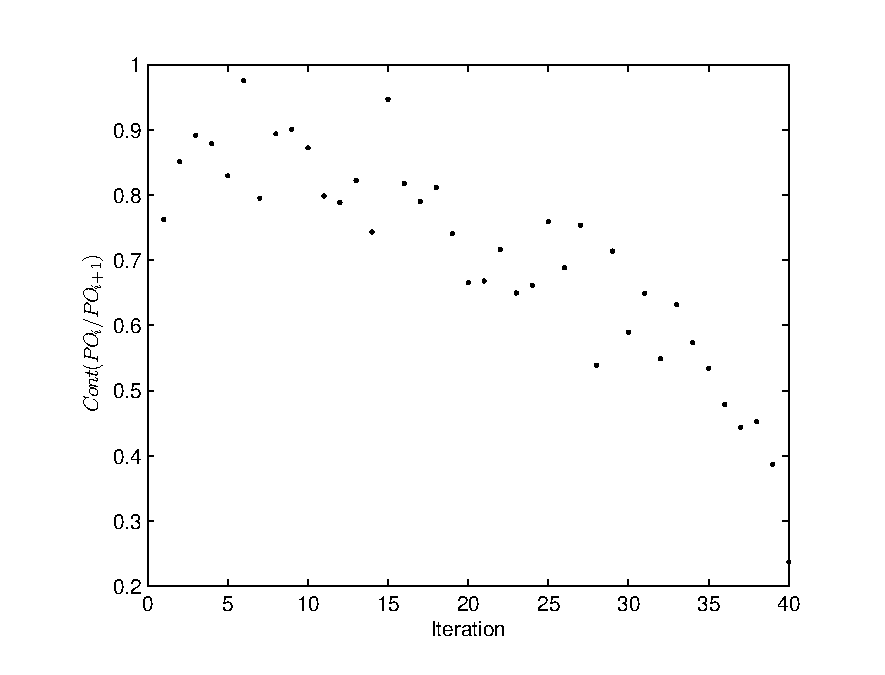
\includegraphics[width=1\linewidth]{contrib2new.eps}
\end{center}
\vspace{-0.5cm}
\caption{Evolution of the contribution indicator}
\label{fig:contrib}
\end{figure}

\section{Spread indicator}
\label{app:spread}

The spread indicator $I_s$ combines the distribution and cardinality to measure the dispersion of the approximated Pareto set $A$:
\begin{equation}
I_s = \frac{\sum_{u \in A}|\{u' \in A: \|F(u)-F(u')\|>\sigma\}|}{|A|-1}
\end{equation}
where $F(u)$ is a fitness function and $\sigma > 0$ a neighborhood parameter. The closer is the measure to 1, the better is the spread of the approximated set $A$.

The Figure \ref{fig:spread_indicator} shows the results of the spread indicator $I_s$ function of the neighborhood indicator $\sigma$ (all the 5 experiments share the same graph shape). We see that the Pareto front is well spread: if  we consider $I_s \geq 0.9$ we have $\sigma < 0.35$ in average for the 5 runs (normalized values), so we can consider that the algorithm produces a well-spread approximation of the Pareto front.
%Knowing that the extreme (Euclidean) distance between two solutions is equal to 332 (for normalized values), we can consider that the algorithm produces a well-spread approximation of the Pareto front.

\begin{figure}[h!]
\begin{center}
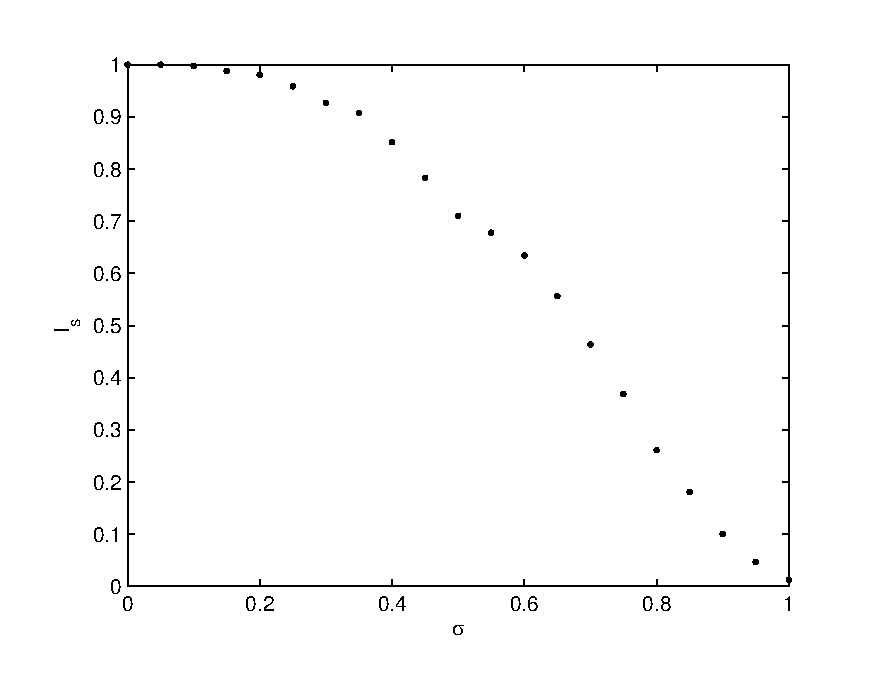
\includegraphics[width=1\linewidth]{spread_indicator_norm2.eps}
\end{center}
\vspace{-0.5cm}
\caption{Spread indicator $I_s$ function of the neighborhood parameter $\sigma$}
\label{fig:spread_indicator}
\end{figure}

\section{Binary $\epsilon$-indicator}
The binary $\epsilon$-indicator is a convergence-based indicator. It will give the quality of a solution front in comparison with a another set, with regards to all objectives. Let us consider a minimization problem with $n$ positive objectives. An objective vector $f^1 = (z_1^1, z_2^1, \dots, z_n^1)$ is said to $\epsilon$-dominate another objective vector $f^2 = (z_1^2, z_2^2, \dots, z_n^2)$ if $\forall 1 \leq i \leq n : \: z_i^1 \leq \epsilon \cdot z_i^2$, for a given $\epsilon > 0$. A binary $\epsilon$-indicator $I_\epsilon(A,B)$ gives the factor $\epsilon$ such that for any solution in $B$ there is at least one solution in $A$ that is not worse by a factor of $\epsilon$ in all objectives. $I_\epsilon(A,B)$ can be calculated as follows \cite{1197687}:
\begin{equation}
I_\epsilon(A,B) = \max\limits_{z^2 \in B} \: \min_{z^1 \in A} \: \max_{1 \leq i \leq n} \: \frac{z_i^1}{z_i^2}
\end{equation}

The reference set $R$ computed from all the experiments will serve to show the evolution of the $\epsilon$-indicator over time. This evolution is shown in Table \ref{tab:biepsref} (for averaged values after each 10 iterations). We can see that in the first iterations, $I_\epsilon(A,R) > 1$ and $I_\epsilon(R,A) \approx 1$ which means that the front is improved while in the last iterations, $I_\epsilon(A,R) > 1$ and $I_\epsilon(R,A) > 1$ which shows convergence.

A comparison of the binary $\epsilon$-indicators between each experiment is also given, in Table \ref{tab:biepsxp}. We can see that $I_\epsilon(A,B) > 1$ and $I_\epsilon(B,A) > 1$ which indicates that neither $A$ weakly dominates $B$ nor $B$ weakly dominates $S$. This means that the generated front is consistent from one experiment to another.

Also, in Table \ref{tab:biepsiter} are given the $\epsilon$-indicator between iterations of an experiment (the same observations apply for the other runs). We can see that in the first iterations, the front is always improved ($I_\epsilon(A_i, A_{i-1}) > 1$ and $I_\epsilon(A_{i-1}, A_i) \leq 1$) while in the last iterations, it begins to converge ($I_\epsilon(A_i, A_{i-1}) > 1$ and $I_\epsilon(A_{i-1}, A_i) > 1$).

\begin{table}[h!]
\begin{center}
\begin{small}
\begin{tabular}{|c|c|c|}
\hline Iteration & Averaged $I_\epsilon(A,R)$ & Averaged $I_\epsilon(R,A)$\\
\hline 1 & 5.5255 & 1.0178\\
\hline 10 & 4.4307 & 1.0235\\
\hline 20 & 3.8102 & 1.1023\\
\hline 30 & 2.3614 & 1.1234\\
\hline 40 & 1.6569 & 1.2381\\
\hline
\end{tabular}
\end{small}
\end{center}
\caption{Evolution of the binary $\epsilon$-indicator (averaged values compared to the reference set $R$) over time}
\label{tab:biepsref}
\end{table}

\begin{table}[h!]
\begin{center}
\begin{footnotesize}
\begin{tabular}{|c|c|c|c|c|c|}
\hline $I_\epsilon(A,B)$ & Run 1 & Run 2 & Run 3 & Run 4 & Run 5 \\ 
\hline Run 1 & 1 & 1.7270 & 1.3594 & 1.8664 & 1.2542 \\ 
\hline Run 2 & 1.5713 & 1 & 1.4122 & 1.7791 & 1.3420 \\ 
\hline Run 3 & 1.4737 & 1.8638 & 1 & 1.9268 & 1.3069 \\ 
\hline Run 4 & 1.3436 & 1.4564 & 1.2843 & 1 & 1.2365 \\ 
\hline Run 5 & 1.4214 & 1.7650 & 1.3918 & 1.7545 & 1 \\ 
%\hline Run 1 & 1 & 1.7234 & 1.3772 & 1.8880 & 1.2152 \\ 
%\hline Run 2 & 1.5305 & 1 & 1.3548 & 1.8333 & 1.3488 \\ 
%\hline Run 3 & 1.4409 & 1.9285 & 1 & 1.8305 & 1.2952 \\ 
%\hline Run 4 & 1.3709 & 1.4048 & 1.2654 & 1 & 1.2310 \\ 
%\hline Run 5 & 1.4554 & 1.8533 & 1.4400 & 1.7868 & 1 \\ 
\hline 
\end{tabular} 
\end{footnotesize}
\end{center}
\caption{Comparison of the binary $\epsilon$-indicators for each experiment}
\label{tab:biepsxp}
\end{table}

\begin{table}[h!]
\begin{center}
\begin{tabular}{|c|c|c|}
\hline Iteration & $I_\epsilon(A_i, A_{i-1})$ & $I_\epsilon(A_{i-1}, A_i)$ \\ 
\hline 1 & 1.6674 & 1.1053 \\ 
\hline 2 & 1.7223 & 1 \\ 
\hline 3 & 2.4439 & 1 \\ 
\hline 4 & 1.7477 & 1 \\ 
\hline 5 & 2.0577 & 1 \\ 
\hline \dots & \dots & \dots \\
\hline 38 & 1.8788 & 1.4916 \\
\hline 39 & 1.5344 & 1.8065 \\ 
\hline 40 & 1.9862 & 1.6609 \\
\hline 
\end{tabular} 
\end{center}
\caption{Comparison of the binary $\epsilon$-indicators between iterations of the same experiment}
\label{tab:biepsiter}
\end{table}

\section{Unary hypervolume indicator}
The hypervolume is an hybrid indicator. Since we already used a binary indicator (\textit{epsilon}), we will use the hypervolume indicator $I_H$ in its unary form. $I_H$, associated with an approximation set $A$ is given by the volume of the space portion that is weakly dominated by the set $A$ \cite{talbi09}.

The evolution of the hypervolume (averaged values) is given in Table \ref{tab:hypervolref} and in Figure \ref{fig:hypervolref}. We can see that the value is (linearly) increasing over time.

The result for each experiment is also given, in Table \ref{tab:hypervol} and the used reference point is the worst point computed from all the sets for normalized data. As we can see, the values are rather consistent from one run to another.

\begin{table}[h!]
\begin{center}
\begin{tabular}{|c|c|}
\hline Iteration & Averaged hypervolume \\
\hline 1 & 0.0574 \\
\hline 10 & 0.0701 \\
\hline 20 & 0.0876 \\
\hline 30 & 0.0931 \\
\hline 40 & 0.1036 \\
\hline
\end{tabular}
\end{center}
\caption{Evolution of the unary hypervolume indicator (averaged values compared to the reference set $R$) over time}
\label{tab:hypervolref}
\end{table}

\begin{figure}[h!]
\begin{center}
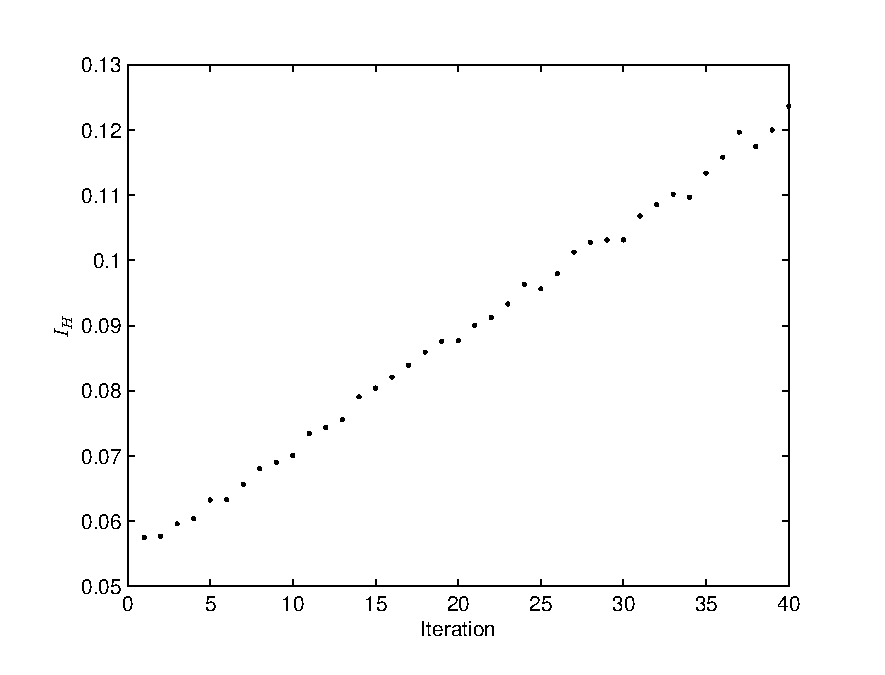
\includegraphics[width=1\linewidth]{hypervolref.eps}
\end{center}
\vspace{-0.5cm}
\caption{Evolution of the unary hypervolume indicator (averaged values compared to the reference set $R$ over time}
\label{fig:hypervolref}
\end{figure}

\begin{table}[h!]
\begin{center}
\begin{tabular}{|c|c|}
\hline Run & $I_H$\\
\hline 1 & 0.1171\\
\hline 2 & 0.1105\\
\hline 3 & 0.1015\\
\hline 4 & 0.1185\\
\hline 5 & 0.0939\\
%\hline 1 & 0.084617\\
%\hline 2 & 0.084566\\
%\hline 3 & 0.094522\\
%\hline 4 & 0.102438\\
%\hline 5 & 0.101421\\
\hline 
\end{tabular}
\end{center}
\caption{Hypervolume for each experiment}
\label{tab:hypervol}
\end{table}

\section{Density of the Pareto front - gaps in the frontier}
Another indicator of the Pareto front structure is its density. Here we will measure the density by finding gaps in the frontier. This will be done by counting the number of solutions in the neighborhood of another solution. Since the extreme distance between two solutions is 450.364 in average for the 5 runs (non-normalized), we consider that an acceptable neighborhood is twice the distance between two solutions if all the solutions were equidistant. We have thus a neighborhood of about 2. This test has shown that there was always at least one solution near another one, even for a neighborhood of 1, meaning that the algorithm can produce a sufficiently dense frontier.

%\subsubsection*{Binary hypervolume indicator}
%The binary hypervolume indicator $I_{H2}(A,B)$ is defined as the hypervolume of the subspace that is weakly dominated by $A$ but not by $B$. A value closer to 0 means that $B$ is a better approximation \cite{1197687}.

%\subsection{Convexity indicator}
%The convexity is also an indicator of the structure. Globally, the Pareto front is not convex, as one may expect since the heterogeneous nature of the criteria. However, the frontier appear to be partially convex and this convexity also depends on the set of criteria that are considered. This is probably due to some correlation between the criteria but this is still to be investigated more deeply since the convexity properties can have an impact on the choice of the multicriteria method to use.

%\section{General properties of the algorithm}
\section{Conclusion}
In this chapter, we have shown that the proposed methodology has proved to be robust even if the problem contains criteria of heterogeneous nature. With the several indicators that we have analysed, we can conclude that the algorithm we used can show good properties of convergence, spread and density.
%For information purposes, we have also computed less state-of-the-art indicators: the contribution indicator and the spread indicator, as defined in \cite{talbi09}. These results are presented in Appendices \ref{app:cont} and \ref{app:spread} and we can see that they also reflects the good convergence and diversity of the algorithm.

Also, analyses have been performed to determine the shape of the Pareto front. Globally, the Pareto front is not convex, as one may expect since the heterogeneous nature of the criteria. This is probably due to some correlation between the criteria but this is still to be investigated.

In the next chapter, we will show how these results can be exploited, with a multi-criteria point of view, to help a designer.

%\section{Conclusion}
%
%In this chapter we have shown that the used methodology has proved to be robust even if the problem contains criteria of heterogeneous nature.

%With these results, we believe that a multi-criteria paradigm can be applied to the design of 3D-SICs in order to produce them more efficiently than what can be done with the current tools.

%Globally, our methodology includes two steps:
%\begin{itemize}
%\item Fast design space exploration and performance estimation/optimization using metaheuristics
%\item Ex-post exploration for multi-criteria decision analysis and decision over the most-suitable solutions
%\end{itemize}
%This work has focused on the first step. As future works, the second step is still to be done. Indeed, now that we can generate a Pareto front, we have to fully analyze how the information provided by the frontier can be used by a designer with an ex-post exploration. As for the criteria, they will be improved continuously in order to be able to have more accurate estimation.

%It is worth to stress that we have done this work for a real case study but it will also be interesting to see how this methodology can be used on other structures, especially when there is a scaling effect on the number of components. Finally, this research will be validated by integration to existing design flow such as PathFinding \cite{DBLP:conf/3dic/MilojevicCCRRSAPM09}. This will allow us to work with a complete flow, from architecture/system-level to physical design and to compare this methodology with the current classical ones.

%These two processes constitute a research field on their own and will need extensive future works. For instance, if many criteria are involved, it can be long and difficult to efficiently establish the Pareto frontier since many of the explored solutions can be efficient solutions, as highlighted in~\cite{Farina02, Stanojevic08}. Also, a graphical decision space might be unusable with many criteria since no relevant information can be visualized, as shown in~\cite{Stanojevic08}. These issues are being studied and one promising way to overcome them is to integrate the preference model in the solution space exploration process~\cite{1569979, Branke04, Cvetkovic00}. In addition, the establishment of a preference model of a designer in relation with several criteria is another research field which also constitute a future work.

%We believe that with these promising results of our first approach, it will be possible to efficiently design 3D-SICs using MCDA tools.
